\chapter{Population Dynamics Epidemiology}
In the following we will study models to simulate the behavior of the
demographic of the populations and/or the transfer process into the 
body. These dynamics could be represented with a deterministic approach
using Ordinary differential equations (ODEs).
\section{Compartmental models}
\textbf{Compartmental models} refers to a class of models where the 
overall population can be partitioned in separate, non-overlapping 
compartments.

This models are useful to analyze dynamics of individuals within, and 
across, compartments.

An example of Compartmental model is the \textbf{Susceptible, Vaccinated, 
Infected, Recovered} (SIRV) Model.

\begin{figure}[!ht]
    \centering
    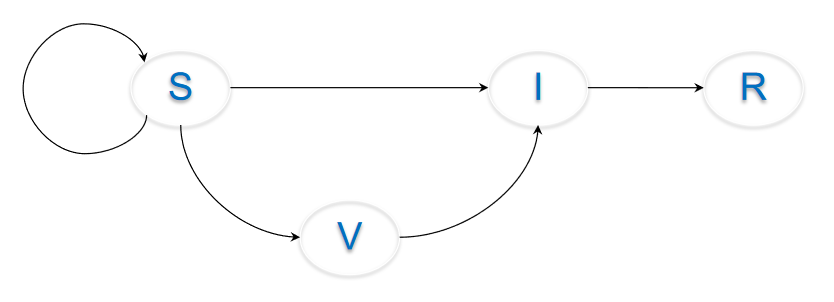
\includegraphics[width=0.5\linewidth]{img/SIRV.png}
    \caption{Susceptible, Vaccinated, Infected, Recovered model}
    \label{fig:sirv}
\end{figure}

\section{Kermack-McKendrick Epidemic Model}
The most basic epidemiological model was formulated by was first proposed 
by Kermack and McKendrick in 1927; this is a compartments model with 3 
classes:
\begin{itemize}
    \item $S(t)$ is the class of individuals who are healthy but can 
        contract the disease: these are called \textbf{susceptible} individuals;
    \item $I(t)$ is he class of individuals who have contracted the 
        disease and are now sick with it, called \textbf{infected} individuals;
    \item $R(t)$ is the class of individuals who have recovered and 
        cannot contract the disease again are called \textbf{removed/recovered} 
        individual;
\end{itemize}

\begin{figure}[!ht]
    \centering
    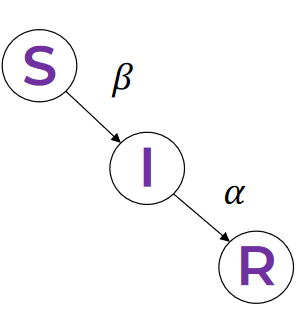
\includegraphics[width=0.25\textwidth]{img/SIR.png}
    \caption{Kermack-McKendrick Epidemic Model}
    \label{fig:SIR}
\end{figure}

This model is based on the following constraint:
\begin{enumerate}
    \item We suppose that each individual of a population could be 
        assigned into nonintersecting classes;
    \item It is assumed that infected individuals are also infectious;
    \item The number of individuals N in the population is fixed
        \begin{equation*}
            N = S(t) + I(t) + R(t)
        \end{equation*}
\end{enumerate}

Also, as we've seen in other simulation models we need to define the 
parameters. In this case, we have the following transition rates among 
the compartments.
\begin{itemize}
    \item $C$ is the probability for an individual to make a contact in 
        a unit of time (per capita contact rate);
    \item $C N$ is the total number of contacts per unit of time;
    \item $S/N$ is the probability that a contact is with a susceptible 
        individual;
    \item $C N (S/N)$ is number of contacts with susceptible individuals 
        of one infectious individual;
    \item $p$ is the probability that a contact with a susceptible 
        individual results in transmission;
    \item $p C S$ is number of susceptible individuals who become 
        infected per unit of time, per infectious;
    \item $p C S I$ is the number of individuals who become infected 
        per unit of time;
    \item Definition: $pC = \beta$ transmission rate constant;
\end{itemize}

Given that $\beta$ is defined as transmission rate constant, we can now 
state that:
\begin{equation}
    S'(t) = \beta I(t) S(i)
\end{equation}
Those individuals who recover or die leave the infected class at constant 
per capita probability recovery per unit of time $\alpha$, called the 
recovery rate. Hence, we have the following equations:
\begin{equation}
    I'(t) = \beta I(t)S(t) - \alpha I(t)
\end{equation}
\begin{equation}
    R'(t) = \alpha I(t)
\end{equation}

The SIR model have the following properties:
\begin{enumerate}
    \item The number of susceptible individuals is constantly declining;
    \item The number of recovered individuals is always increasing;
    \item The number of infected individuals increases if the following holds:
    \begin{equation*}
        \frac{\beta S(0)}{\alpha} > 1
    \end{equation*}
\end{enumerate}

Now, If we assume that there are no deaths or births in the population, we can solve
the differential equation as follow:
\begin{equation}
    \begin{array}{lc}
        S'(t) = & - \beta \frac{I(t)S(t)}{N} \\ 
        I'(t) = & \beta \frac{I(t)S(t)}{N} - \alpha I(t) \\
        R'(t) = & \alpha I(t)
    \end{array}
\end{equation}

Let's also consider to following ratio:
\begin{equation*}
    R_0 = \frac{\beta}{\alpha}
\end{equation*}
This number is called the \textbf{basic reproduction number} (or ratio). 
The number tells us what is the expected insurgence of “new” infections 
in a population where $S(0) = N - I(0), R(0) = 0$ and $I(0) = I_{initial}$

Whether $R_0 > 1$ or $R_0 < 1$ tells us how fast the disease is spreading.

The numbers $\beta$ and $\alpha$ can be thought of as rate constants of
yielding the expected times of infection (through a contact) and the time 
to recovery.
\begin{equation*}
    T_c = \frac{1}{\beta} \, \, \, T_r = \frac{1}{\alpha}
\end{equation*}

Solving the set of equations leads to the following relation:
\begin{equation}
    I(t) + S(t) - \frac{\alpha}{\beta} \ln (S(t)) = C
\end{equation}
Given initial conditions $I(0)$ and $S(0)$, the relation also holds 
for $t = 0$ and $t = \infty$.

From the rewriting of the equation for the number of infected people $
I(0)$, we can observe the following:
\begin{itemize}
    \item $R_0 S(0) > N \implies I'(0) > 1$
    \item $R_0 S(0) < N \implies I'(0) < 1$
\end{itemize}
Which tells us how important it is to establish the value of $R_0$.
\subsection{Variations on the SIR Model}
\begin{itemize}
    \item The Susceptible-Infected-Susceptible model (SIS) is used to 
        model diseases like the standard flu.
        \begin{figure}[!ht]
            \centering
            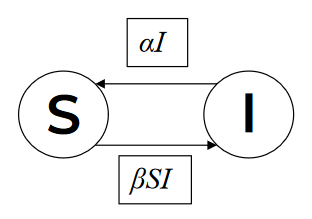
\includegraphics[width=0.25\linewidth]{img/SIS.png}
            \caption{Susceptible-Infected-Susceptible model}
            \label{fig:SIS}
        \end{figure}
    \item In the Susceptible-Infected-Removed-Deceased model (SIRD) a 
        new possible outcome is included: the possibility of death given an infection;
       \begin{figure}[!ht]
            \centering
            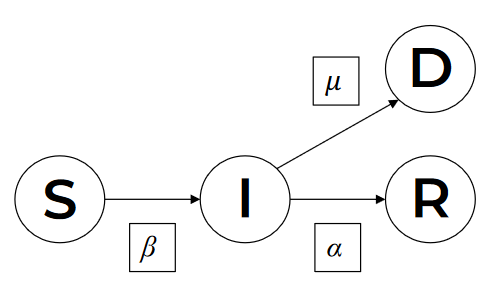
\includegraphics[width=0.25\linewidth]{img/SIRD.png}
            \caption{Susceptible-Infected-Removed-Deceased model}
            \label{fig:SIRD}
        \end{figure}
   \item The simplest one introduces a population of vaccinated (V) which           reduces the pool of susceptible people.
        \begin{figure}[!ht]
            \centering
            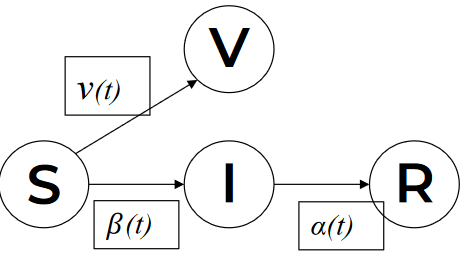
\includegraphics[width=0.25\linewidth]{img/SIRV1.png}
            \caption{Simplest one introduces a population of vaccinated}
            \label{fig:SIRV1}
        \end{figure}
\end{itemize}
\section{Network models}
Network models look at the spreading of an epidemics at an individual 
level and do not represent the populations as a compartment.

These methods represent either individuals or metapopulations, i.e., 
spatially separated groups of similar individuals, as a node of a complex 
network-

The contacts (the possible paths of transmission of the disease) are the 
edges of this network.